\section{Products and Results}

As products of this project, we developed a software composedof two scripts:
\begin{itemize}
	\item \textbf{generate\_composition} receives two parameters:
	\begin{enumerate}
		\item set how many children (partners) each node will have;
		\item set the depth of the tree
	\end{enumerate}
	\item \textbf{send\_messages} receives 6 parameters:
	\begin{enumerate}
		\item the host in which the service is;
		\item the port to reach the service;
		\item the service path from the root of the host;
		\item the size, in bytes, of each message that will be sent to the composition;
		\item the frequency, number of messages per second, in which the script will send the message to the composition;
		\item how many times the batch of messages will be sent
	\end{enumerate}
\end{itemize}

This system is licensed under GPL.

\subsection{Results}
We managed to execute the composition on ``Revoada'', a LAN inside IME-USP, consisting in eight machines. With a maximum of eight nodes we were able to generate three designs of topologies, which we called:

\begin{itemize}
	\item \textbf{Balacend Tree}, a balanced binary tree with depth of 2 (forcibly, by our infrastructural constraints, it has only 7 nodes);
	\item \textbf{Vertical Tree}, a tree with each node having just one child, and depth varying from 2 to 7 (using a minimum of 3 and a maximum of 8 nodes);
	\item \textbf{Horizontal Tree}, one root node with 2 to 7 Leaf nodes as children, depth fixed on 1 (using a minimum of 2 and a maximum of 8 nodes)
\end{itemize}

Graphical examples of these topologies are shown in Figure \ref{trees}

\begin{figure}[htb]
	\centering
	\subfigure[The only option for a Balanced Tree in ``Revoada'']{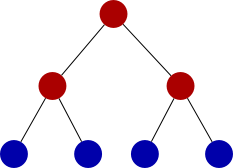
\includegraphics[width=0.3\textwidth]{images/balanced-tree}} \qquad
	\subfigure[Vertical Tree]{
\includegraphics[trim = -40mm 0mm -40mm 0mm, height=0.5\textwidth]{images/vertical-tree}} \\
	\subfigure[Horizontal Tree]{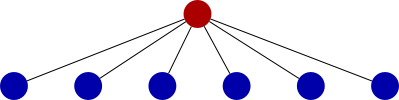
\includegraphics[width=0.5\textwidth]{images/horizontal-tree}}
	\caption{Example trees for each topology available in ``Revoada''}%
	\label{trees}
\end{figure}


To be ``fair'' to the comparison of the tests, we stablished that each of the trees would have 7 nodes, this means a ``vertical tree'' with depth of 6, the ``balanced tree'', and a ``horizontal tree'' with 6 children.

For the scalability analysis we have chosen the method ``$2^k$ factorial''. This method uses two levels for each factor of the experiment to determine the influence of them on the response time of the composition. Our controllable factors are the \emph{size} of each message and the \emph{frequency} to send the messages to the system, so we chose $1 kB$ (one kilobyte) and $1 MB$ (one megabyte) for the size and $10$ (ten) and $100$ (one hundred) messages per second for the frequency.

With these values, we ran the script (``send_messages'') four times, one for each combination of the chosen values, for each of the three topologies. The results, simplified to show only the real time execution and its statistics, are shown next.

\lstinputlisting{images/compiled-results.txt}
	
With the averages we are finally able to calculate the influence effect of each factor for each topology. We have done this with a predefined algebraic process, first let $I$ be the mean case, $A$ be the effect of frequency of messages and $B$ be the effect of message size. Then let

\begin{center}
	\begin{tabular}{c | r l}
		\multirow{2}{*}{$x _A = $} & -1 & if 10  messages per second \\
		                           &  1 & if 100 messages per second \\
	\end{tabular}
\end{center}

\begin{center}
	\begin{tabular}{c | r l}
		\multirow{2}{*}{$x _B = $} & -1 & if 1kB message size \\
		                           &  1 & if 1MB message size \\
	\end{tabular}
\end{center}

Then we have the model: $y = q _I + q _A x _A + q _B x _B + q _AB x _A x _B $, where $y$ is, in our case, the real time acquired from the experiment. The interpretation will be:
\begin{itemize}
	\item[$q _I$] is the Mean Real Time
	\item[$q _A$] is the effect of Frequency of messages
	\item[$q _B$] is the effect of message Size
	\item[$q _AB$] is the interaction between Frequency of messages and message Size
\end{itemize}

To solve the linear system generated by the substitution of $y$, $x _A$, and $x _B$, we used the ``Sign Table Method'' [\citet{2KFACTORIAL}]. The tables used can be found next:

\begin{table}[h]
	\caption{Sign Table to determine the influence effect of each factor in ``Balanced Tree''}
	\rowcolors{1}{lightgray}{white}
	\center
	\begin{tabular}{ c c c c r }
		\hline
		I & A & B & AB & Real Time \\
		\hline
		1 & -1 & -1 &  1 &    9.01 s \\
		1 &  1 & -1 & -1 &   90.06 s \\
		1 & -1 &  1 & -1 &  186.98 s \\
		1 &  1 &  1 &  1 & 1876.71 s \\
		\hline
		2162.78 & 1770.78 & 1964.62 & 1608.66 & Total \\
		540.69 & 442.69 & 491.15 & 402.16 & Total/4 \\
		\hline
	\end{tabular}
\end{table}
\begin{table}[h]
	\caption{Sign Table to determine the influence effect of each factor in ``Vertical Tree''}
	\rowcolors{1}{lightgray}{white}
	\center
	\begin{tabular}{ c c c c r }
		\hline
		I & A & B & AB & Real Time \\
		\hline
		1 & -1 & -1 &  1 &   13.32 s \\
		1 &  1 & -1 & -1 &   28.81 s \\
		1 & -1 &  1 & -1 &  276.38 s \\
		1 &  1 &  1 &  1 & 2022.55 s \\
		\hline
		2341.06 & 1761.65 & 2256.79 & 1730.68 & Total \\
		585.26 & 440.41 & 564.19 & 432.67 & Total/4 \\
		\hline
	\end{tabular}
\end{table}
\begin{table}[h]
	\caption{Sign Table to determine the influence effect of each factor in ``Horizontal Tree''}
	\rowcolors{1}{lightgray}{white}
	\center
	\begin{tabular}{ c c c c r }
		\hline
		I & A & B & AB & Real Time \\
		\hline
		1 & -1 & -1 &  1 &   18.00 s \\
		1 &  1 & -1 & -1 &  192.11 s \\
		1 & -1 &  1 & -1 &  250.00 s \\
		1 &  1 &  1 &  1 & 2199.07 s \\
		\hline
		2659.19 & 2123.19 & 2238.96 & 1774.96 & Total \\
		664.79 & 530.79 & 559.74 & 443.74 & Total/4 \\
		\hline
	\end{tabular}
\end{table}

Now that we have the effect of each variable, we need to discover what is the \emph{variation explained} of each factor, so that we can realize the importance of each factor. There is another algebraic way to calculate this variation: $Total = 2^2 * q _A ^2 + 2^2 * q _B ^2 + 2^2 * q _AB ^2  $, where each element of the summation is the variation of the related factor. Finally we apply this calculations for each topology:

\begin{center}
	\begin{tabular}{ | c | l | }
		\hline
		\multirow{4}{*}{Balanced Tree}& Total variation $= 2395811.71$ \\
		                              & Variation of Frequency $= 783920.85 (32.72\%)$ \\
		                              & Variation of Size $= 964937.26  (40.28\%)$ \\
		                              & Variation of Intersection $= 646953.59 (27.00\%)$\\
		
		\hline
		\multirow{4}{*}{Vertical Tree} & Total variation $= 3167847.20$ \\
		                               & Variation of Frequency $= 1126984.03 (35.57\%)$ \\
		                               & Variation of Size $= 1253237.38 (39.57\%)$ \\
		                               & Variation of Intersection $= 787625.78 (24.86\%)$\\ 
		
		\hline
		\multirow{4}{*}{Horizontal Tree} & Total variation $= 2797959.71$ \\
		                                 & Variation of Frequency $= 775860.63 (27.73\%)$ \\
		                                 & Variation of Size $= 1273284.26 (45.51\%)$ \\
		                                 & Variation of Intersection $= 748814.81 (26.76\%)$\\
		\hline
	\end{tabular}
\end{center}

